%! Author = Yan Wittmann

\chapter{Projektbericht} \label{ch:projektbericht}

In der Einleitung (Kapitel\ \ref{sec:projektbericht-projektziel}) wird zunächst auf die Abteilung im Unternehmen, die aktuelle Situation und die Ziele für das Projektsemester eingegangen.
Bei den darauf folgenden Grundlagen (Kapitel\ \ref{sec:projektbericht-grundlagen}) werden die relevanten Themen, Begriffe und Standards erklärt.
Wie die Praktikumsziele erreicht wurden, wird im Lösungsweg detailliert (Kapitel \ref{sec:projektbericht-loesungsweg}).

\section{Einleitung, Problemstellungen und Projektziel} \label{sec:projektbericht-projektziel}

Die für dieses Praktikum relevante Abteilung in der {\metaeffekt} stellt ein automatisiertes Vulnerability Monitoring bereit und integriert es bei diversen Kunden, deren Wünsche und Anforderungen priorisiert in die Systeme zurückgeführt werden.
Das Vulnerability Monitoring wird intern durch eine Aneinanderreihung von Prozessschritten modelliert, die auch als \qt{Inventory Enrichment Pipeline} bezeichnet wird.
Die Prozessschritte erhalten jeweils ein Software-Inventar als Eingabe, welches sie auf eine bestimmte definierte Weise modifizieren und für den nächsten Schritt bereitstellen, sodass ein Inventar, das alle Schritte durchlaufen hat, alle nötigen Schwachstell-Informationen angereichert bekommen hat.
Auf diese Pipeline wird im Kapitel\ \ref{subsec:projektbericht-grundlagen-vulnerability-monitoring} kurz eingegangen, sie soll allerdings nicht Hauptbestandteil dieses Berichts sein und dient nur zur besseren Einordnung der anderen Prozesse.

In dem Praktikum liegt der Schwerpunkt vor allem auf dem CVSS-Standard\textsuperscript{\ref{subsec:projektbericht-grundlagen-cvss}}, insbesondere in der Verbesserung unseres Supports für neuere Versionen dieses und in konzeptionelle Änderungen, wie das System mit diesen umgehen sollte.
Konkret geht es um die folgenden Punkte:

\begin{smitemize}
    \item Über die Monate vor dem Praktikum ist es bereits immer deutlicher geworden, dass das Datenmodell hinter dem Vulnerability Monitoring fast komplett neu geschrieben werden muss, um neue Anforderungen und Erkenntnisse effizient und korrekt unterstützen zu können.
    Die relevante Anforderung an das Datenmodell ist es, die Art und Weise, wie die CVSS-Vektoren abzulegen und verarbeitet werden, komplett neu zu planen und zu schreiben.
    Es wurde erkannt, dass meistens nicht nur ein CVSS-Vektor einer Quelle pro Schwachstelle (CVE, \ldots) vorhanden ist, sondern mehrere, die von mehreren Organisationen und Institutionen vergeben werden, da ihre Meinungen über den Schweregrad voneinander abweichen können.
    Bisher wird mit diesen zusätzlichen Vektoren nicht bewusst unterschiedlich umgegangen, es wird einfach der erste verarbeitet, der vorhanden ist.
    Um diese Situation zu verbessern, soll ein System eingeführt werden, das über die einzelnen Schritte der Inventory Enrichment Pipeline nur die Vektoren aggregiert und noch nicht verarbeitet oder berechnet.
    Erst zum Ende, wenn es darum geht die Reports (PDF, HTML) zu generieren, sollen die Vektoren ausgewählt, eventuell kombiniert und deren Scores berechnet werden.
    Bei dem Überarbeiten des Datenmodells muss also darauf geachtet werden, diese Anforderung zu unterstützen.
    Zudem muss ein CVSS-Selektor geschrieben werden, der die darzustellenden Vektoren berechnen kann.
    \item Zuletzt ging es noch um die Implementierung des CVSS-Standards in TypeScript, die Open Source gestellt werden sollte und mit einem Web-UI als online verfügbarer, interaktiver CVSS-Rechners verfügbar sein soll.
    Dieser soll dann aus den eigenen Reports verlinkt werden können.
    Der Grund hierfür ist simpel: Es gibt bisher keinen online CVSS-Rechner, der alle unsere Anforderungen erfüllt.
    Es gibt keinen Rechner, der alle Versionen zugleich unterstützt, keinen, der mehrere Vektoren gleichzeitig gut vergleichbar zulässt und leider haben viele der offiziellen Rechner auch Probleme, die URL-Parameter korrekt zu erkennen.
\end{smitemize}

In diesem Bericht wird ein Fokus auf die CVSS-seitigen Arbeiten im Unternehmen gelegt, da sie den Großteil des Semesters eingenommen haben.


\section{Grundlagen} \label{sec:projektbericht-grundlagen}

\subsection{Software-Inventare} \label{subsec:projektbericht-grundlagen-inventories}

Software-Inventare werden bei der {\metaeffekt} in einem eigens entwickelten, proprietären Format, schlicht \qt{Inventar} genannt, abgelegt.
Meist wird, um ein solches Inventar zu erhalten, ein ebenfalls eigens entwickelter Scanner verwendet, der ganze Dateisysteme nach Komponenten durchsucht und daraus ein Inventar generiert.
Um möglichst breiten Support zu bieten, gibt es allerdings nicht nur den Scanner, sondern auch diverse Konverter, mit denen Inventare von und zu Formaten wie CycloneDX SBOM\footnote{\url{https://cyclonedx.org/specification/overview}} oder SPDX\footnote{\url{https://spdx.dev}} umgewandelt werden können.

Diese Inventare können mehrere Kategorien an Daten enthalten: Software-Komponenten (\qt{Artefakte}), Schwachstell-Informationen, Security Advisories, Lizenzinformationen und einige weitere.

\subsection{NVD / NIST} \label{subsec:projektbericht-grundlagen-nvd-nist}

Software-Schwachstellen sind allgegenwärtig, jedes Softwareprodukt hat sie und meistens es ist nur eine Frage der Zeit, bis sie gefunden, veröffentlicht und im schlimmsten Fall ausgenutzt werden.
Die National Vulnerability Database (NVD)\footnote{\url{https://nvd.nist.gov}} des National Institute of Standards and Technology (NIST) der U.S.\ Regierung stellt mit ihrem CVE-System\textsuperscript{\ref{subsec:projektbericht-grundlagen-cve-cpe}} eine der primären Quellen für Schwachstell-Informationen für Forscher, Unternehmen und automatisierte Tools bereit.
Sobald eine neue Schwachstelle bekannt gegeben wird, nehmen sie diese in ihren Katalog an CVE mit auf, versehen sie mit CVSS- und Matching-Informationen über das CPE-System.
Damit ist die Schwachstelle für alle auf der Welt über eine API oder über ihr User Interface erreichbar und kann, falls ein Projekt betroffen ist, frühzeitig kontextualisiert bewertet werden.

\subsection{CVE / CPE} \label{subsec:projektbericht-grundlagen-cve-cpe}

\qt{CVE} ist ein von dem CVE Project eingeführtes System, das Schwachstellen in Software- und Hardwareprodukten eindeutig identifiziert und beschreibt.
Der Standard wird stark von der NVD des NIST unterstützt.
Im CVE-System bekommt jede Schwachstelle, die von einem Forscher oder einer Organisation gefunden und veröffentlicht wird, eine eindeutige ID von der Form \qt{CVE-YYYY-NNNN} zugewiesen, wobei \qt{YYYY} das Jahr der Veröffentlichung und \qt{NNNN} eine eindeutige, fortlaufende Nummer ist.
CVE definiert eine Schwachstelle als:

\begin{quote}
    A weakness in the computational logic (e.g., code) found in software and hardware components that, when exploited, results in a negative impact to confidentiality, integrity, or availability.
    Mitigation of the vulnerabilities in this context typically involves coding changes, but could also include specification changes or even specification deprecations (e.g., removal of affected protocols or functionality in their entirety).
    \cite{nvdVulnerabilityDefinition}
\end{quote}

Eine Schwachstelle ist also eine Schwäche, eine theoretische Angriffsfläche, die durch Ausnutzen negative Auswirkungen auf die Vertraulichkeit, Integrität oder Verfügbarkeit eines Systems hat.
Es soll kein CVE-Eintrag existieren, der keinen Einfluss auf die Vertraulichkeit, Integrität oder Verfügbarkeit eines Systems hat \cite{nvdVulnerabilityMetrics}.

Jeder CVE werden gewisse Metadaten zugeordnet, wie Beschreibungen, Referenzen und (potenziell mehrere) CVSS-Vektoren zur Bewertung des Schweregrads, aber auch \qt{CPE}s, die Aussagen über die betroffenen Produkte machen und automatisierte Zuordnungen erlauben.
Common Platform Enumeration (CPE) ist ein von der MITRE Corporation\footnote{\url{https://cpe.mitre.org/specification}} entwickeltes System, mit dem Soft- und Hardwareprodukte über den Hersteller, Produktnamen und Version eindeutig identifiziert werden können.
Die CPE Naming Specification Version 2.3 \cite[Seite 37, Kapitel 6.2]{NISTIR7695} definiert die Syntax eines CPE-Strings, in der mindestens \qt{part} (Komponenten-Typ), \qt{vendor} (Hersteller) und \qt{product} (Produkt) gesetzt sein müssen:

\code{cpe : 2.3 : part : vendor : product : version : update : edition}\newline\hphantom{\code{cpe}}\code{: language : sw_edition : target_sw : target_hw:other}

Auf dem NVD Dashboard\footnote{\url{https://nvd.nist.gov/general/nvd-dashboard}} ist gelistet, dass es am 08.03.2024 insgesamt 240899 eindeutige CVEs und 1261617 CPEs gibt.
Diese Zahl wächst exponentiell und zeigt, wie wichtig es ist, Schwachstellen automatisiert zu verarbeiten.

\subsection{CVSS} \label{subsec:projektbericht-grundlagen-cvss}

Das Common Vulnerability Scoring System (CVSS) wird in Version 4.0 \cite{CVSSv4.0Specification} vom FIRST\footnote{\url{https://www.first.org}} (Forum of Incident Response and Security Teams) als ein offener Standard für die Bewertung der Sicherheitsanfälligkeit von Software- und Hardwarekomponenten beschrieben.
Dieser Standard legt fest, wie sog\. CVSS-Vektoren, definiert als Sammlung von Schlüssel-Wert Paaren, zur möglichst objektiven Darstellung von Schwachstelleneigenschaften genutzt werden können.
Solche Vektoren können textuell als \code{CVSS:VERSION/KEY:VALUE/KEY:VALUE/...} formatiert werden, wobei jedes Wertepaar durch \qt{/} getrennt und mit \qt{CVSS:} gefolgt von der Vektor-Version beginnen muss.

Ein Beispiel für einen Basisvektor in Version 3.1, der einen mittleren Schweregrad (\qt{Medium}) mit einem Score von 6.0 darstellt, kann folgendermaßen aussehen: \code{CVSS:3.1/AV:L/AC:L/PR:H/UI:N/S:U/C:H/I:H/A:N}.
Allgemein reichen die Scores, die aus diesen Vektoren berechnet werden, von 0 bis 10 und ordnen die Schwachstellen in die Kategorien \qt{Low}, \qt{Medium}, \qt{High} und \qt{Critical} ein, wobei höhere Werte eine dringendere Bewertung erfordern.
Diese Berechnungen lassen sich leicht mit Online-Rechnern\footnote{\url{https://metaeffekt.com/security/cvss/calculator}} oder Software-Tools, verfügbar in allen populären Programmiersprachen, durchführen.

Die versionsabhängigen Metriken der Vektoren ordnen jeweils eine Charakteristik einer Schwachstelle einem Wert zu.
So steht beispielsweise \code{AV:L} für einen \qt{Attack Vector} mit dem Wert \qt{Adjacent Network}, was die räumliche Nähe beschreibt, die ein Angreifer benötigt, um die Schwachstelle auszunutzen.
Andere Werte wie \qt{Network} (aus dem Internet ausnutzbar, höchster Schweregrad), \qt{Local} oder \qt{Physical} (physikalischer Zugang benötigt, am weigsten schlimm) spezifizieren weitere Angriffsszenarien für diese Metrik.

Zusätzlich zu den allgemeinen, umgebungsunabhängigen Basismetriken, die von den Herausgebern der Schwachstelleninformationen festgelegt werden, gibt es noch die \qt{Temporal}/\qt{Threat}- und \qt{Environmental}-Metriken.
Diese Metriken reflektieren die spezifische Umgebung und den Kontext, in dem eine Schwachstelle existiert, und werden in betroffenen Projekten von den Anwendern kontextabhängig gesetzt.
Damit erlaubt es CVSS, eine initiale, kontextunabhängige Bewertung eines Systems, und durch Hinzufügen von Kontextinformationen auch eine kontextualisierte Sicht auf das System zu erhalten.
Einer Schwachstelle können von verschiedenen Parteien potenziell mehrere, unterschiedliche Vektoren zugeordnet werden, dieser Aspekt wird später wichtig.

\subsection{Automatisiertes Vulnerability Monitoring} \label{subsec:projektbericht-grundlagen-vulnerability-monitoring}

Das bei der {\metaeffekt} eingesetzte automatisierte Vulnerability Monitoring, hat das Ziel, für ein gegebenes Software-Inventar nicht nur die relevanten Schwachstellen (\qt{Vulnerabilities}) zu identifizieren, sondern auch zugehörige Ratgeber (\qt{Security Advisories}) als Hilfestellung zu der darauf folgenden manuellen Bewertung bereitzustellen.
Der Prozess, dargestellt in Grafik \ref{fig:vulnerability-monitoring-overview-figure}, in zwei Hauptphasen mit mehreren Unterschritten gegliedert, wird im Folgenden beschrieben.
Als Eingabe dient in jedem Fall ein Inventar gefüllt mit einer Liste an Software-Komponenten und deren Metadaten, wie Version, Quelle und Ökosystem-spezifischen Informationen.

Der erste Prozessschritt ist die Identifikation von Schwachstellen und wird getrennt voneinander auf alle Komponenten im Inventar angewandt.
Die in unserem Prozess verwendeten externen Schwachstellendatenbanken nutzen abstrahierte Darstellungen von Produkten und Software-Komponenten für ihre internen Verweise zwischen Produkten und Schwachstellen.
Beispielsweise verwendet die NVD CPEs (siehe Kapitel \ref{subsec:projektbericht-grundlagen-cve-cpe}), GitHub Security Advisories\footnote{\url{https://github.com/advisories}} folgen dem OSV-Schema\footnote{\url{https://osv.dev}} mit Ökosystem-abhängigen Informationen, und Microsoft (MSRC)\footnote{\url{https://msrc.microsoft.com/update-guide}} arbeitet mit numerischen Identifikatoren, die nur durch Download und Extraktion aller monatlichen Zusammenfassungen über ihre API zugänglich sind.
Die Zuordnung unserer realen Komponenten zu diesen abstrahierten Produkten stellt daher immer eine Herausforderung dar.
Unser Vulnerability Monitoring setzt verschiedene Algorithmen ein, um diese Zuordnungen so weit wie möglich automatisch vorzunehmen, was jedoch nicht immer fehlerfrei gelingt.
Falsch positive und falsch negative Ergebnisse erfordern dann eine manuelle Korrektur durch einen gepflegten Datensatz (\qt{Korrelationsdaten}), was einen erheblichen Zeitaufwand bedeutet.

Wenn dieser Schritt erfolgreich abgeschlossen ist, können Abfragen an die jeweiligen Datenbanken gestartet werden, um Schwachstellen durch Produkt- und Versionsabgleichen zu identifizieren.
Dieses Zwischeninventar mit Schwachstellinformationen kann bereits für Berichte genutzt werden, jedoch wird meistens ein weiterer Schritt dahinter geschaltet:
Weitere Abfragen an einen größeren Satz an Datenbanken werden gestartet, um zu den gefundenen Schwachstellen entsprechende Ratgeber zuzuordnen.
Diese Abfragen sind in der Regel einfacher, da die Ratgeber-Einträge meistens direkt auf die betroffenen Schwachstellen-IDs Bezug nehmen.
Das Ergebnisinventar kann dann als Grundlage für die Erstellung von Reports und Statistiken benutzt werden.

\begin{figure}[htbp] % here, top, bottom, separate page
    \centering
    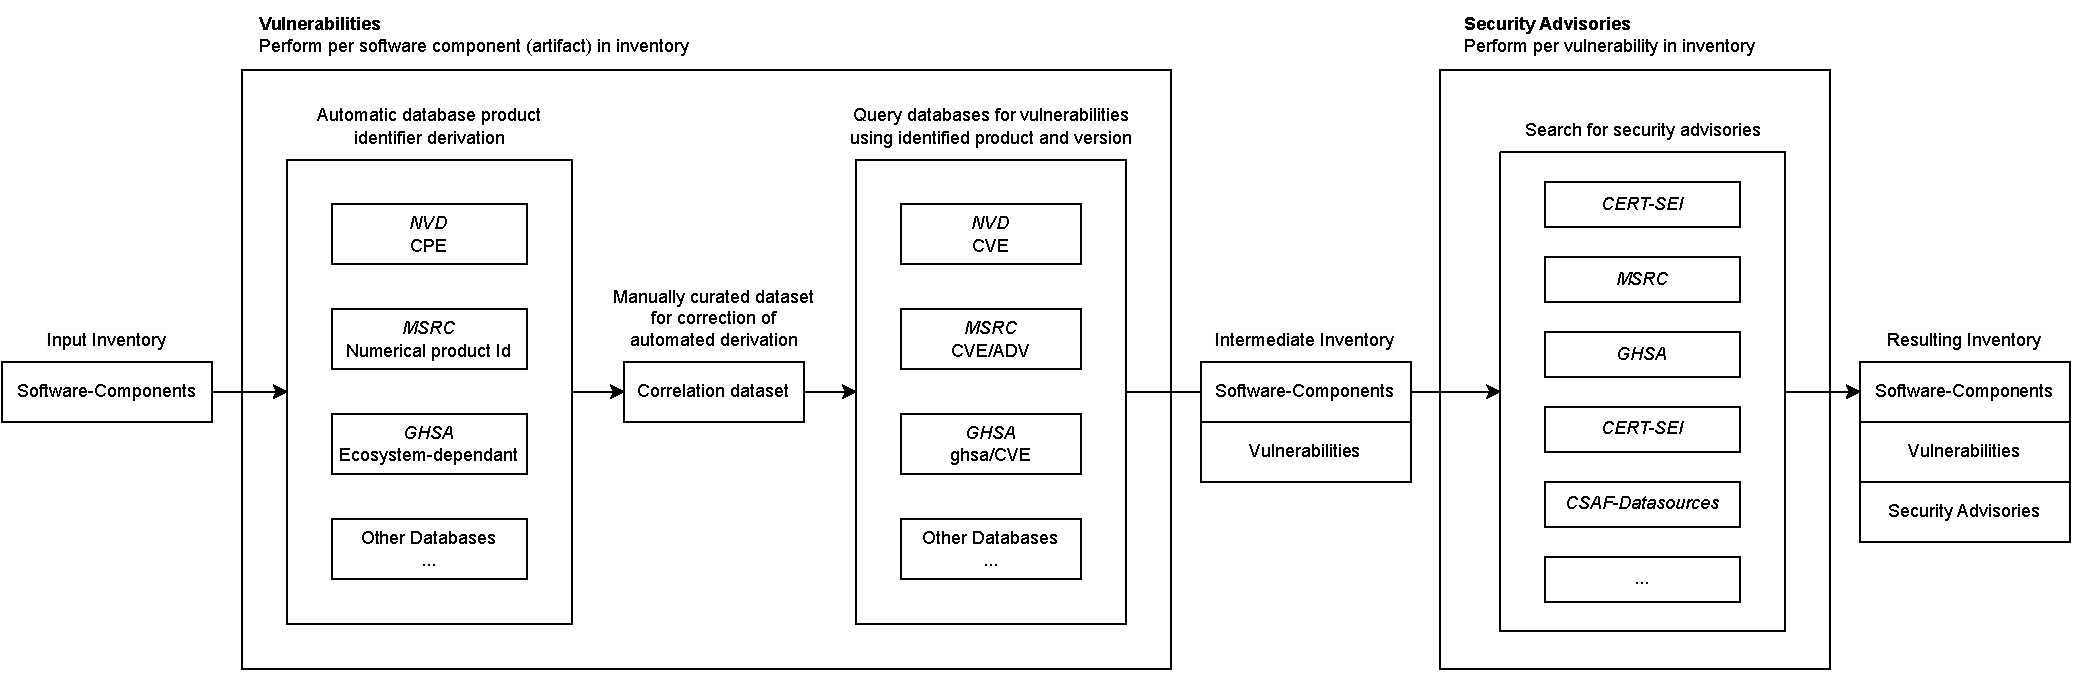
\includegraphics[width=1\textwidth, keepaspectratio]{res/grafiken/vulnerability-monitoring-overview}
    \caption{Schwachstellsuche mit einem Software-Inventar}
    \label{fig:vulnerability-monitoring-overview-figure}
\end{figure}

\subsection{Schwachstellen-Priorisierung durch CVSS} \label{subsec:projektbericht-grundlagen-vulnerability-assessment}

Wenn eine Liste an Schwachstellen durch den Prozess in \ref{subsec:projektbericht-grundlagen-vulnerability-monitoring} als Minimalanforderung in einem Projekt für ein Inventar erfasst wurde, muss nun ein zweiter Schritt folgen:
Die manuelle Bewertung der Schwachstellen, indem eine Einschätzung, ein Status und erforderliche Maßnahmen angegeben werden.
Jedoch kann es sowohl bei großen, aber auch schon bei kleinen Projekten mit kritischen Abhängigkeiten zu einer großen Menge an Schwachstellen kommen (1000 und aufwärts), die oftmals nicht alle sofort von einer Person oder einem Bewertungs-Team durchgearbeitet werden können.
Es werden also objektive und automatisierbare Faktoren benötigt, anhand denen die Schwachstellen möglichst ohne weiteres Zutun in eine priorisierte Liste eingeordnet werden können, um die kritischsten zuerst abarbeiten zu können.

Diese Faktoren sind Projekt- und Umgebungsspezifisch und können stark variieren.
In diesem Kapitel wird nur CVSS als Priorisierungsfaktor betrachtet, wie sie in der CVSS-Spezifikation beschrieben werden \code{[TODO: CITATION NEEDED]}.
In Kapitel \ref{subsec:projektbericht-grundlagen-cvss} wurde bereits auf die Metrik-Gruppen eingegangen.
Da jede Schwachstelle aus dem CVE-System und den meisten anderen Systemen mindestens einen CVSS-Vektor von den Herausgebern angehängt bekommen hat, kann bereits ohne großen Mehraufwand eine nach dem daraus errechneten Basis-Score sortierte Liste als initiale Reihenfolge dienen.

Vor allem die Environmental-Metrikgruppe kann nun zur Kontextualisierung von Schwachstellen in einem Projekt verwendet werden.
Das Beispiel bezüglich des \qt{Attack Vector}s in \ref{subsec:projektbericht-grundlagen-cvss}, bei dem \code{AV} auf \code{L} kann hier weiter getrieben werden:
Wenn eine aus einem lokalen Netzwerk ausnutzbare Schwachstelle in einer Applikation vorhanden ist, die keinerlei Netzwerkzugang hat, dann kann diese auch nicht aus einem Netzwerk ausgenutzt werden, sondern eventuell nur durch physikalischen Zugriff.
Allgemein kann dann also eine globale, Inventar-weite CVSS-Vektoränderung von \code{AV:P} angewendet werden, aus der eine neue, kontextualisierte Liste an Schwachstellen hervorgeht, die nun akkurater die tatsächlichen Risiken eines Systems darstellen.
Weitere Metriken wie das Risiko eines Verlusts an Konfidentialität, Integrität oder Verfügbarkeit können für weitere Anpassungen verwendet werden.


\section{Lösungsweg} \label{sec:projektbericht-loesungsweg}

In diesem Kapitel werden die Problemstellungen in verschiedenen Schritten als Lösungsweg beschrieben.

\subsection{CVSS-Vektor Quellenmanagement} \label{subsec:projektbericht-loesungsweg-cvss-source-management}

Im Kontext der zuvor diskutierten Grundlagen stößt man unweigerlich auf die Herausforderung, mehrere voneinander abweichende CVSS-Vektoren für eine einzige Schwachstelle zu handhaben.
Ein System zur Verwaltung dieser Vektoren ist daher notwendig, das nicht nur mehrere Vektoren der gleichen Version zulässt, sondern diesen auch die ursprüngliche Quelle und weitere Metadaten mit hoher Eindeutigkeit anhängen kann.
Zudem muss die Serialisierung und Deserialisierung der Informationen sowohl in einem menschenlesbaren Format, als auch maschinenlesbaren möglich sein.
Eine weitere Anforderung ist es, die Quellen der Vektoren auch dann noch nachvollziehen zu können, wenn mehrere Vektoren miteinander kombiniert wurden.
Dessen Konzeption berücksichtigte eine Vielzahl von Quellen, wie unter anderem:

\begin{itemize}
    \item NVD:
    Organisationen und Institutionen können, wenn sie als sogenannte CVE Naming Authorities (CNA) registriert sind, für CVEs beliebige CVSS-Vektoren veröffentlichen.
    Eine öffentlich verfügbare Liste an CNAs ist online\footnote{\url{https://nvd.nist.gov/vuln/cvmap/search}} mit Metadaten verfügbar.
    \item Microsoft Security Response Center (MSRC):
    Sie stellen für jede für Microsoft relevante Schwachstelle und pro betroffene (numerische) Produkt-Id einen CVSS-Vektor zur Verfügung.
    \item CERT-SEI und GitHub Security Advisories (GHSA): Stellen jeweils einen Vektor pro referenzierter Schwachstelle zur Verfügung.
\end{itemize}

Aus den abgeleiteten Anforderungen wurde das in Listing \ref{lst:cvss-source-format} abgebildete Format für Vektor-Quellen entworfen, wobei jede der drei Zeilen eine der alternativen Optionen darstellt.
Eine Quelle besteht $immer$ $mindestens$ mit der \qt{CvssVersion} aus einer Vektor-Version und einer \qt{HostingEntity}, die die Entität darstellt, die den Vektor auf ihrer Platform zur Verfügung stellt.
Eine Entität kann sich z.B.\ auf die NVD, MSRC, GHSA, usw.\ beziehen.
Wenn die \qt{HostingEntity} nicht die Entität ist, die den Vektor initial zur Verfügung gestellt hat, dann muss dieser Herausgeber als \qt{IssuingEntity} zusätzlich gesetzt sein.
In gewissen externen Schwachstelldatenbanken werden die Issuing Entities unter definierten Rollennamen geführt, wie die CNAs bei der NVD\@.
In diesem Fall muss auch die \qt{IssuerRole} angegeben werden.

Die Darstellung dieser Quelleninformationen in einer Datenstruktur erfolgt einfach durch separate Attribute und kann einfach z.B.\ als JSON serialisiert werden.
Für die Serialisierung als menschen- aber auch maschinenlesbarer String müssen jedoch einige Regeln definiert werden.
Vom Konzept her wird einfach das Format aus Listing \ref{lst:cvss-source-format} verwendet; um allerdings die bereits definierten Bindestriche als Trennzeichen weiterhin verwenden zu können, müssen eventuelle Bindestriche (\qt{-}) in Entitäten und Rollenbezeichnern durch \qt{\textbackslash-} ersetzt werden und alle \qt{\textbackslash} durch \qt{\textbackslash\textbackslash}, um Konflikte zu vermeiden.
Das Fehlen von Leerzeichen in CVSS-Versionen erlaubt die einfache Trennung der Version von den übrigen Elementen mittels des ersten Leerzeichens.

\begin{lstlisting}[language={}, label={lst:cvss-source-format}, caption={Alternative CVSS-Quellen Formatdefinitionen}]
CvssVersion HostingEntity
CvssVersion HostingEntity-IssuingEntity
CvssVersion HostingEntity-IssuerRole-IssuingEntity
\end{lstlisting}

Zur Unterstützung kombinierter Vektoren und Quellen wird das Format um die Möglichkeit erweitert, mehrere Quellen mittels der Zeichenfolge \qt{ + } zu trennen, wie in Listing \ref{lst:cvss-source-format-combined} dargestellt.
Plus-Zeichen (\qt{+}) innerhalb der Quellen müssen daher auch entsprechend als \qt{\textbackslash+} kodiert werden.
Trotz der Kombination verschiedener Quellen ist $nur$ $eine$ Angabe der CVSS-Version nötig, da eine Kombination von Vektoren unterschiedlicher Versionen von Grund auf nicht möglich ist.
Die Reihenfolge der Quellen ist dennoch von Bedeutung, da die erste Quelle den Basisvektor darstellt und folgende Quellen in der angegebenen Reihenfolge auf diesen angewandte Modifikationen sind.

Listing \ref{lst:cvss-source-format-examples} zeigt beispielhafte Quellenangaben.
Dieses Format wird im weiteren Verlauf, speziell in Kapitel \ref{subsec:projektbericht-loesungsweg-cvss-selection}, als Grundlage für die Verwaltung und Auswahl von CVSS-Vektoren dienen.

\begin{lstlisting}[language={}, label={lst:cvss-source-format-combined}, caption={CVSS-Quellen Format \(Kombiniert\)}]
CvssVersion HostingEntity-IssuerRole-IssuingEntity + HostingEntity-IssuerRole-IssuingEntity + ...
\end{lstlisting}

\begin{lstlisting}[language={}, label={lst:cvss-source-format-examples}, caption={CVSS Sources Format}]
CVSS:3.1 Microsoft Corporation
CVSS:2.0 Assessment-all
CVSS:2.0 NVD-CNA-NVD
CVSS:3.1 NVD-CNA-Microsoft Corporation
CVSS:4.0 Assessment-lower
\end{lstlisting}

Als Zusatz zu diesem System ist für die Zuordnung von Metadaten wie E-Mail-Adressen oder URLs zu den jeweiligen Entitäten ist der Aufbau eines Datensatzes der bekannten Quellen erforderlich.
Ein dafür entworfener automatisierter Prozess, der auf die Inhalte von CVE.org\footnote{\url{https://www.cve.org/PartnerInformation/ListofPartners}} zugreift, erstellt regelmäßig eine lokale Liste und speichert diese in mehreren JSON-Dateien.
Dazu wird ein zusätzlicher Datensatz gepflegt, um auch Entitäten zu unterstützen, die nicht in dieser Liste geführt werden.


\subsection{CVSS-Vektor Selektion} \label{subsec:projektbericht-loesungsweg-cvss-selection}

Mit dem Format aus Kapitel \ref{subsec:projektbericht-loesungsweg-cvss-source-management} werden ab Generation 3 des Vulnerability Monitorings der {\metaeffekt} ALLE Vektoren zu den gefundenen Schwachstellen mit in das Inventar der Komponenten aufgenommen.
Generation 2 dieses Systems hat diese Multiplizität der Vektoren einfach übergangen.
Da die Auswahl der effektiven Vektoren als Nebeneffekt des zuständigen Codes durch ein \qt{First-Come-First-Serve}-Verfahren realisiert war, wurde eine bewusste Entscheidung der Kunden von Anfang an ausgeschlossen.
Um zu jedem Zeitpunkt die genaue Quelle eines Vektors nachvollziehbar zu halten, werden bei dem neuen System zunächst alle Vektoren über den Prozessverlauf aggregiert und erst in den Schritten ausgewertet werden, in denen sie interpretiert werden müssen.
Die Funktionsweise der CVSS-Vektor-Selektion wird in diesem Kapitel erklärt.

Vor Beginn ist konzeptionell erneut zu betonen, dass die Auswahl der, von den vorhergegangenen Prozessschritten angesammelten, Vektoren wirklich erst ab den Schritten geschieht, in denen sie auf egal welcher Art und Weise dargestellt oder für weitere Berechnungen benötigt werden.
Die Selektion bezieht sich immer auf die Vektoren einer einzigen, vollständigen Schwachstelle.
Dieser Prozess wird in zwei Teile geteilt, da für einige Use-Cases bereits das Zwischenergebnis von Interesse ist.

Ein Schritt, der vor der Auswahl stattfinden muss, ist es, erst die relevanten Vektoren einer Schwachstelle zu sammeln.
Hierfür gibt es einige Fälle die beachtet werden müssen:
Natürlich werden alle Vektoren, die direkt auf der Schwachstelle sind, direkt hinzugefügt.
Einige Vektoren werden nicht von der Schwachstelle selbst, sondern von referenzierten Security Advisories beigetragen, also müssen auch diese eingesammelt werden.
Doch nicht immer sind alle Vektoren anwendbar, zum Beispiel bei Vektoren von Microsoft gibt es Bedingungen, wann ein Vektor anwendbar ist.
Diese Bedingungen müssen hier erst ausgewertet werden, wodurch Vektoren eventuell herausgefiltert werden.
Zudem kann es sein, dass ein projektinternes Bewertungsteam eigene Vektoren für eine Schwachstelle vergeben hat, diese müssen natürlich auch berücksichtigt werden.

Um die Einordnung des Themas zu vereinfachen, wird dieser Prozess beispielhaft in Schaubild \ref{fig:cvss-selection-process-collection} mit dem Betriebssystem \qt{Windows 10 Pro} mit frei erdachten, jedoch realistischen Schwachstellen, Security Advisories und Vektor-Quellen durchgeführt.
\ifshortenedReport
Dieses betroffene Betriebssystem durchläuft als Komponente die Inventory Enrichment Pipeline, und bekommt damit die gefundenen Schwachstellen und Security Advisories angehängt.
\else
Dieses betroffene Betriebssystem durchläuft als Komponente die Inventory Enrichment Pipeline, wie in Kapitel \ref{subsec:projektbericht-grundlagen-vulnerability-monitoring} beschrieben, und bekommt damit die gefundenen Schwachstellen und Security Advisories angehängt.
\fi
Nicht nur die Schwachstelle und die Security Advisories wurden mit CVSS-Vektoren versehen, sondern gab es auch mehrere Vektor-Modifikationen von manuellen Bewertungen als \qt{Assessment}-Vektoren.
Das Beispiel wird in Kapitel \ref{subsubsec:projektbericht-loesungsweg-cvss-selection-example} mit der Selektion der Vektoren weitergeführt.

\begin{figure}[htbp] % here, top, bottom, separate page
    \centering
    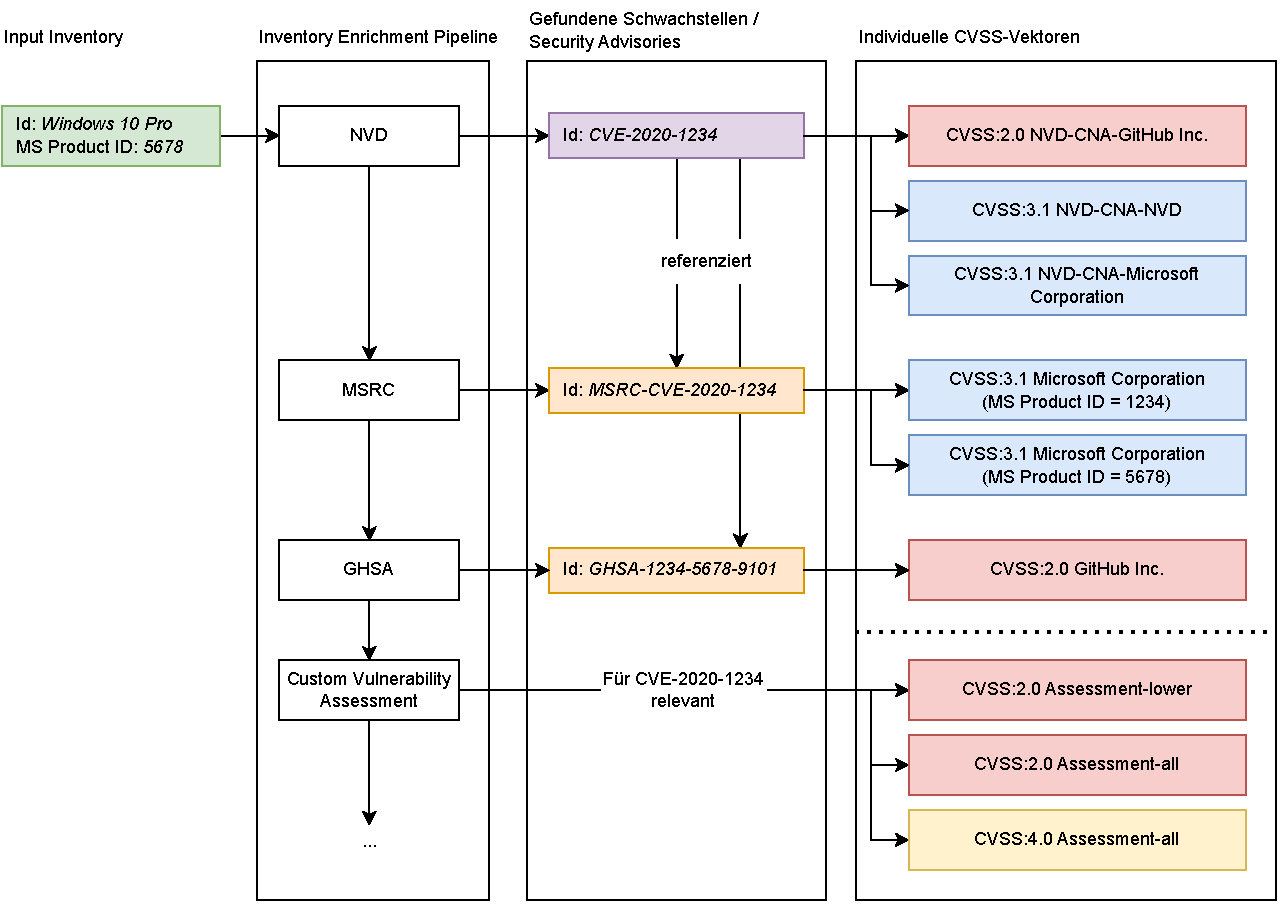
\includegraphics[width=1\textwidth, keepaspectratio]{res/grafiken/cvss-selection-process-collection}
    \caption{Beispiel: Initialer Zuordnungs- und Sammelungsschritt für Schwachstelldaten und CVSS-Vektoren}
    \label{fig:cvss-selection-process-collection}
\end{figure}

Nachdem alle Vektoren angesammelt wurden, kann die Selektion gestartet werden, die, wie bereits erklärt, in zwei Teile aufgeteilt ist.
Wichtig ist zudem, dass der Auswahlprozess in der Realität zwei Mal stattfinden muss, einmal für einen \qt{initial} und einen \qt{context} Selektor.
Der Grund dafür ist, dass es für Kunden wichtig ist, die Nachvollziehbarkeit, welcher Vektor und Score von den externen Datenquellen gekommen ist und wie sie diesen durch ihre \qt{assessment}-Vektormodifikationen verändert haben.

\begin{enumerate}
    \item
    Nutze einen Selektor, um aus allen aggregierten Vektoren eine reduzierte Menge zu bilden, die pro Version nur einen Vektor enthält.
    Diese Vektoren werden für Radardiagramme als Übersicht und zur Aufschlüsselung der unterschiedlichen Einschätzungen und Interpretationen zwischen den Versionen verwendet.
    Dieser Schritt macht den Hauptteil der Berechnungslogik aus, da er hoch anpassbar sein soll.
    \item
    Eine weitere Regel wird dann auf diesem ersten Ergebnis benutzt, um zwischen den unterschiedlichen Versionen zu entscheiden und einen als effektiven Vektor für die Schwachstelle zu bestimmen.
    Dieser wird für die Repräsentation der Schwachstelle in weiteren Diagrammen und Tabellen verwendet, da eine Differenzierung zwischen Versionen auf solch einem höheren Betrachtungslevel nicht sinnvoll oder relevant ist.
\end{enumerate}

\subsubsection{Schritt 1: Selektionsregeln} \label{subsubsec:projektbericht-loesungsweg-cvss-selection-rules-1}

Allgemein ist der Selektionsschritt in drei Abschnitte aufteilbar.
Der erste sucht in potenziell mehreren Schritten, definiert durch gekapselte Regeln, Vektoren aus der aggregierten Menge an Vektoren heraus und kombiniert diese auf eine definierbare Weise.
Die darauffolgenden beiden Schritte dienen zur Auswertung des Ergebnisvektors, um diesen eventuell noch einmal zu manipulieren oder etwa in bestimmten Situationen gar keinen zurückzugeben.

Ein Auszug der relevanten Klasse mit ihren Attributen, die für die Selektion aus Schritt 1 zuständig sind, kann in Listing \ref{lst:cvss-selector-class-attributes} gefunden werden.
Der volle Quellcode mit der vollen Logik kann auf dem öffentlichen Repository\footnote{\url{https://github.com/org-metaeffekt/metaeffekt-core/blob/24a26dd37ab6f9087e2fdc1b338857b404fa835e/libraries/ae-security/src/main/java/org/metaeffekt/core/security/cvss/processor/CvssSelector.java}} gefunden werden.
Eine weitere Anforderung für das dahinterliegende Datenmodell der Selektoren ist es, komplett als JSON-Objekt serialisierbar zu sein, aus dem dann wieder eine identische Java-Objektstruktur aufgebaut werden kann.
Im Quellcode werden darum einige Konvertierungsmethoden zur Verfügung gestellt.

% basicstyle=\tiny
\begin{lstlisting}[language=Java, label={lst:cvss-selector-class-attributes}, caption={CVSS-Selektor Klassen}, basicstyle=\scriptsize]
public class CvssSelector {
    // Die Attribute werden in diesen Unterkapiteln erklaert.
    List<CvssRule> rules; // 1.1
    List<SelectorStatsEvaluator> statsEvaluatorActions; // 1.2
    List<SelectorVectorEvaluator> selectorVectorEvaluators; // 1.3

    public static class CvssRule {
        SourceSelector sourceSelector;
        MergingMethod mergingMethod;
        List<SelectorStatsCollector> statsCollectors;
        List<SelectorVectorEvaluator> vectorEvaluators;
    }
    public static class SourceSelector {
        List<SourceSelectorEntry> preferredSources;
    }
    public static class SourceSelectorEntry {
        List<SourceSelectorEntryEntry<CvssEntity>> hostingEntities;
        List<SourceSelectorEntryEntry<CvssEntity>> issuingEntities;
        List<SourceSelectorEntryEntry<CvssIssuingEntityRole>> issuingEntityRoles;
    }
    public static class SourceSelectorEntryEntry<T extends CvssSource.EntityNameProvider> {
        T value;
        boolean inverted;
    }
    public static class SelectorStatsCollector {
        String attributeName;
        StatsCollectorProvider provider;
        StatsCollectorSetType setType;
    }
    public static class SelectorVectorEvaluator {
        // operations are combined using AND
        // individual operations can be inverted by setting value to true
        Map<VectorEvaluatorOperation, Boolean> operations;
        EvaluatorAction action;
    }
    public static class SelectorStatsEvaluator {
        String attributeName;
        StatsEvaluatorOperation comparator;
        EvaluatorAction action;
        Integer comparisonValue;
    }
    public enum MergingMethod {
        ALL, LOWER, HIGHER, OVERWRITE
    }
    public enum StatsCollectorProvider {
        PRESENCE, ABSENCE, APPLIED_PARTS_COUNT
    }
    public enum StatsCollectorSetType {
        ADD, SUBTRACT, SET, MAX, MIN
    }
    public enum StatsEvaluatorOperation {
        EQUAL, SMALLER, SMALLER_OR_EQUAL, GREATER, GREATER_OR_EQUAL
    }
    public enum VectorEvaluatorOperation {
        IS_NULL, IS_BASE_FULLY_DEFINED, IS_BASE_PARTIALLY_DEFINED, IS_ENVIRONMENTAL_PARTIALLY_DEFINED, IS_TEMPORAL_PARTIALLY_DEFINED, IS_THREAT_PARTIALLY_DEFINED
    }
    public enum EvaluatorAction {
        FAIL, RETURN_NULL, SKIP, RETURN_PREVIOUS
    }
}
\end{lstlisting}

\paragraph{Schritt 1.1: Regeln zur Vektor-Selektion und -Kombination} \label{par:projektbericht-loesungsweg-cvss-selection-rules-1-1}

Zur Selektion (und Kombination) der effektiven Vektoren werden von einem Benutzer eine Menge an Regeln definiert.
Diese legen je fest, welchen Vektor sie auswählen, wie mit Ergebnissen umgegangen werden soll und ob nutzerdefinierte Variablen modifiziert werden sollen.
Zunächst werden die im Code in der Klasse \code{SourceSelector} als \code{SourceSelectorEntry} benannten Regeleinträge erklärt.
Diese Klassen verwendet die Vektor-Quellennotation, wie in Kapitel \ref{subsec:projektbericht-loesungsweg-cvss-source-management} aufgeführt, zur Eingrenzung des Vektors, der ausgewählt werden soll.
Die einzelnen Einträge erlauben es, Hosting- und Issuing-Entities und eine Issuing Role anzugeben, mit Sonderwerten von \qt{*} für das matchen von beliebigen, aber nicht-leeren Werten und \qt{null}, um einen leeren Wert zu verlangen, die gegen jeden Vektor der Eingangsvektoren gehalten werden.
Das Ergebnis kann optional durch einen weiteren Parameter bei jeder Auswertung invertiert werden, um komplexere Abfragen zu erlauben.
Der erste erfolgreiche Eintrag, der einen Vektor findet, wird an die obere Ebene zurückgegeben, was die Definition von fallback-Strategien ermöglicht.

% Horizontal is this instance, vertical is the parameter.
% |       | ANY | value | null |
% |-------|-----|-------|------|
% | ANY   | Y   | Y     | Y    |
% | value | Y   | ==    | N    |
% | null  | N   | N     | Y    |

Wenn von den Selektoren ein Vektor zurückgegeben wurde, wird über eine \code{MergingMethod} definiert, auf welche Art dieser auf den der vorherigen Regel angewendet werden sollte.
Die häufigste Methode ist \code{ALL}, welche einfach alle Metriken, die von dem gefundenen Vektor definiert sind, auf dem vorherigen setzt.
Weitere Optionen sind \code{HIGHER} und \code{LOWER}, welche Metriken nur dann anwenden, wenn der daraus entstehende Vektor einen gleichen oder höheren/niedrigeren Score, je nach Methode, hervorbringt.
Dies ist nützlich bei Assessment-Vektoren (vom Bewertungsteam ausgestellten), die global auf ein gesamtes Inventar zur begründeten Herunterstufung der Schwachstellen angewendet werden sollen, wie, wenn die Applikation vom Internet komplett abgeschirmt ist oder eine andere Metrik für einen Kontext nicht relevant ist.
Die letzte Option ist \code{OVERWRITE}, welche einfach vollständig den vorherigen Vektor durch den neuen ersetzt.

Beim Anwenden dieser Vektoren werden über die \code{SelectorStatsCollector} verschiedene ganzzahlig numerische Statistiken in benutzerdefinierte Variablen für die \qt{Statistics Evaluators} in Schritt 1.2 getrackt.
Beispielsweise kann ein \qt{Statistics Collector} erstellt werden, der trackt, ob ein Vektor von einer gewissen Regel gefunden wurde (präsenz-Check), oder wie viele Metriken von diesem angewandt wurden (also ob der Vektor modifiziert wurde), was bei den Methoden \code{HIGHER} und \code{LOWER} nützlich sein kann.
Diese Variablen werden bis zum Schritt 1.2 gespeichert, bei dem sie ausgewertet werden können.

Zuletzt können pro Regel noch Checks mit \code{SelectorVectorEvaluator} durchgeführt werden.
Diese können Aktionen über \code{EvaluatorAction} auslösen, wie:
den Prozess komplett scheitern zu lassen, einen leeren Vektor zurückzugeben, diese eine Regel zu überspringen oder an der vorherigen Regel abzubrechen.
Diese Checks können optional invertiert werden.

\paragraph{Schritt 1.2: Statistics Evaluators (Statistik-Auswerter)}

Nun, da in Schritt 1.1 (Unterkapitel von \ref{par:projektbericht-loesungsweg-cvss-selection-rules-1-1}) von den Regeln ein einziger, kombinierter Vektor gebaut wurde, können optional einige der \qt{Statistics Collectors} über die \code{SelectorStatsEvaluator} ausgewertet werden.
Hier werden die typischen numerischen Vergleichsmethoden wie größer, kleiner, gleich, und so weiter zur Verfügung gestellt, um auch hier die Aktionen aus \code{EvaluatorAction} ausführen zu können.

\paragraph{Schritt 1.3: Vector Evaluators}

Abschließende Checks auf dem Ergebnisvektor können wieder über die \code{SelectorVectorEvaluator} durchgeführt werden und über \code{EvaluatorAction} Aktionen auslösen, wie bereits in Schritt 1.1 erklärt.

Dieser komplette Prozess wird bei der {\metaeffekt} je einmal pro Vektor-Version (2.0, 3.1, 4.0) mit jeweils zwei Selektoren (initial, context) durchgeführt und ergibt damit kombinatorisch eine Menge von bis zu sechs Vektoren.

\subsubsection{Schritt 2: Versions-Selektionsregeln} \label{subsubsec:projektbericht-loesungsweg-cvss-selection-rules-2}

Dieser Schritt ist wesentlich einfacher als Schritt 1, da er nur noch angeben muss, von welcher Vektor-Version der effektive Vektor gewählt werden soll.
Die verfügbaren Werte sind in Listing \ref{lst:cvss-selector-version-selector} zu sehen.
Es gibt zwei Kategorien, einmal auf die Vektor-Version (mit latest, oldest und den einzelnen version 2, 3 und 4) und einmal auf die Werte der Scores (höchster, niedrigster) bezogenen.
Die zwei Meistverwendeten sind \code{LATEST}, gefolgt von \code{HIGHEST}.

\begin{lstlisting}[language=Java, label={lst:cvss-selector-version-selector}, caption={Gültige Werte für die Versions-Selektion}]
public enum CvssScoreVersionSelectionPolicy {
    HIGHEST, LOWEST, LATEST, OLDEST, V2, V3, V4
}
\end{lstlisting}

Nach Anwenden dieser beiden Schritte ist die Selektion vollständig durchgeführt.
Im folgenden Abschnitt wird diser Prozess anhand eines Beispiels demonstriert.

\subsubsection{Beispiel zur Vektor-Selektion} \label{subsubsec:projektbericht-loesungsweg-cvss-selection-example}

Das Beispiel, begonnen unter Kapitel \ref{subsec:projektbericht-loesungsweg-cvss-selection} im Schaubild \ref{fig:cvss-selection-process-collection}, wird hier mit den aggregierten Vektoren fortgeführt.
Um die Selektion durchzuführen werden die beiden folgenden Selektoren für initial und context verwendet, die dank einer \code{CvssSelector.explain()}-Methode als menschenlesbarer Text dargestellt werden können.
Diese gezeigten und verwendeten Selektoren sind auch die, die als Standard-Werte im Produktionscode\footnote{\href{https://github.com/org-metaeffekt/metaeffekt-core/blob/1f0a1f6ac5e8343e10ea182794faf534bdfb3310/libraries/ae-inventory-processor/src/main/java/org/metaeffekt/core/inventory/processor/report/configuration/CentralSecurityPolicyConfiguration.java\#L568}{\texttt{https://github.com/org-metaeffekt/metaeffekt-core/blob/...}}} eingetragen sind.

\paragraph{Beispiel, CVSS-Selektor \qt{initial}} \label{par:projektbericht-loesungsweg-cvss-selection-example-selector-initial}

Dies ist der Selektor, der im Folgenden als \qt{initial} bezeichnet wird.

\noindent The CVSS Selector contains 1 rule that will be applied in the following order:
\begin{enumerate}[noitemsep]
    \setlist{nolistsep}
    \item The first matching vector is selected: [NVD-CNA-NVD], [Microsoft Corporation-*-*], [NVD-CNA-Microsoft Corporation], [GitHub, Inc.-*-*], [NVD-CNA-GitHub, Inc.], [NVD-*-*], [CERT-SEI-*-*], [not:Assessment-*-*]. From the selected vector, all vector components are applied to the resulting vector.
\end{enumerate}

\paragraph{Beispiel, CVSS-Selektor \qt{context}} \label{par:projektbericht-loesungsweg-cvss-selection-example-selector-context}

Dies ist der Selektor, der im Folgenden als \qt{context} bezeichnet wird.
Er enthält die Basisregel des \qt{initial}-Selektors, und wird durch Regeln bezüglich der Assessment-Vektoren ergänzt, um eine kontextualisierte Sicht zu ermöglichen.

\noindent The CVSS Selector contains 4 rules that will be applied in the following order:
\begin{enumerate}[noitemsep]
    \setlist{nolistsep}
    \item The first matching vector is selected: [NVD-CNA-NVD], [Microsoft Corporation-*-*], [NVD-CNA-Microsoft Corporation], [GitHub, Inc.-*-*], [NVD-CNA-GitHub, Inc.], [NVD-*-*], [CERT-SEI-*-*], [not:Assessment-*-*]. From the selected vector, all vector components are applied to the resulting vector.
    \item If present, the [Assessment-*-all] vector is selected. From the selected vector, all vector components are applied to the resulting vector. The following 1 statistics collector will also be applied to the selected vector:
    \begin{itemize}[noitemsep]
        \item If a vector is returned from the selection, 1 is added to the stats collector attribute [assessment].
    \end{itemize}
    \item If present, the [Assessment-*-lower] vector is selected. From the selected vector, only vector components that lead to a lower or equal score on the resulting vector are applied. The following 1 statistics collector will also be applied to the selected vector:
    \begin{itemize}[noitemsep]
        \item If a vector is returned from the selection, 1 is added to the stats collector attribute [assessment].
    \end{itemize}
    \item If present, the [Assessment-*-higher] vector is selected. From the selected vector, only vector components that lead to a higher or equal score on the resulting vector are applied. The following 1 statistics collector will also be applied to the selected vector:
    \begin{itemize}[noitemsep]
        \item If a vector is returned from the selection, 1 is added to the stats collector attribute [assessment].
    \end{itemize}
\end{enumerate}

\noindent After finishing the CVSS selection, 1 statistics evaluator will be applied to the resulting vector:
\begin{itemize}[noitemsep]
    \setlist{nolistsep}
    \item If the stats collector attribute [assessment] is equal to 0, then no vector is returned.
\end{itemize}
Additionally, 1 vector evaluator will be applied to the resulting vector:
\begin{itemize}[noitemsep]
    \setlist{nolistsep}
    \item If the resulting vector is not base fully defined, then no vector is returned.
\end{itemize}

\paragraph{Beispiel, Schritt 1: Aggregieren der Vektoren} \label{par:projektbericht-loesungsweg-cvss-selection-example-step-1}

Dieser Abschnitt bezieht sich auf Schaubild \ref{fig:cvss-selection-process-selection-1}.

Zunächst muss, als Eingabe für die Selektionsschritte, eine Menge an Vektoren gesammelt werden.
Da sich dieses Beispiel auf die Schwachstelle \qt{CVE-2020-1234} aus dem vorhergegangenen Beispiel bezieht, werden auf jeden Fall alle Vektoren der Schwachstelle selbst und der referenzierten manuellen Bewertungen (\qt{Assessments}) aufgenommen.
Bedingte Vektoren müssen nun noch auf ihre Bedingung geprüft werden:
Microsoft ordnet pro Produkt in ihren Datensätzen nur einen Vektor zu, darum wird der Vektor mit der Beziehung zu \qt{MS Product ID 1234} herausgefiltert, da die Id der verwendeten Komponente \qt{5678} darauf nicht referenziert wird.

\begin{figure}[htbp] % here, top, bottom, separate page
    \centering
    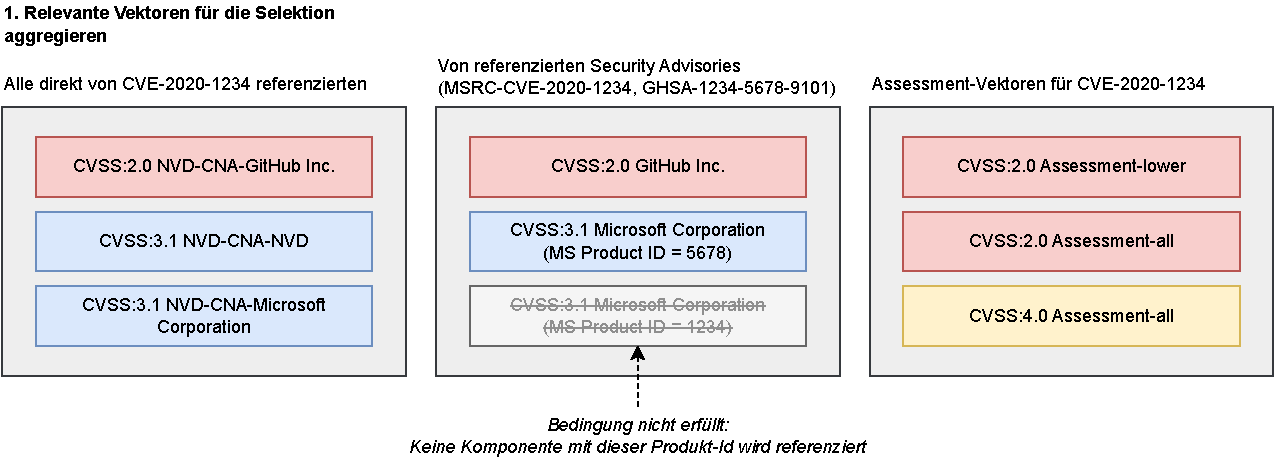
\includegraphics[width=1\textwidth, keepaspectratio]{res/grafiken/cvss-selection-process-selection-1}
    \caption{Aggregierung der CVSS-Vektoren}
    \label{fig:cvss-selection-process-selection-1}
\end{figure}

\paragraph{Beispiel, Schritt 2: Anwenden der CVSS-Selektoren} \label{par:projektbericht-loesungsweg-cvss-selection-example-step-2}

Dieser Abschnitt bezieht sich auf die Schaubilder \ref{fig:cvss-selection-process-selection-2} und \ref{fig:cvss-selection-process-selection-3}.

\begin{figure}[htbp] % here, top, bottom, separate page
    \centering
    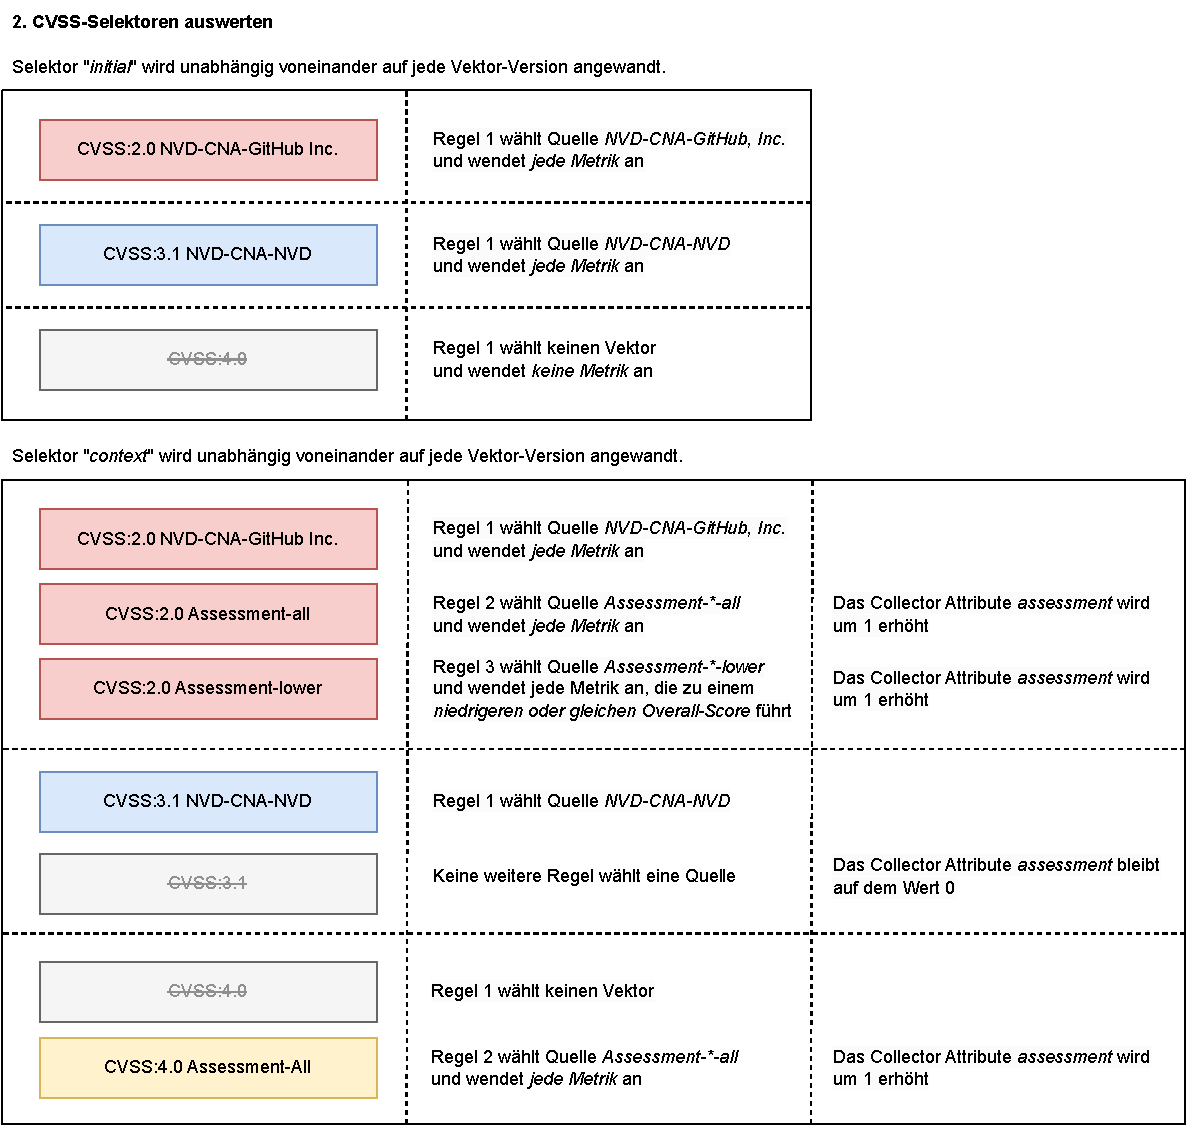
\includegraphics[width=1\textwidth, keepaspectratio]{res/grafiken/cvss-selection-process-selection-2}
    \caption{Auswerten der CVSS-Selektoren}
    \label{fig:cvss-selection-process-selection-2}
\end{figure}

\begin{figure}[htbp] % here, top, bottom, separate page
    \centering
    \includegraphics[width=1\textwidth, keepaspectratio]{res/grafiken/cvss-selection-process-selection-3}
    \caption{Ergebnisse der CVSS-Selektion}
    \label{fig:cvss-selection-process-selection-3}
\end{figure}

Nun können die Selektoren auf die Vektor-Menge angewendet werden.
Im Fall des \qt{initial}-Selektors wird einfach die erste zutreffende Quelle aus der Liste in Regel 1 gewählt.
Außer bei CVSS:4.0 (keine nicht-Assessment-Vektoren) wird hier immer genau ein Vektor zurückgegeben.

Bei dem \qt{context}-Selektor werden genau dieselben initialen Vektoren zunächst ausgewählt, bei CVSS:2.0 wird allerdings noch von den anderen Regeln 2 und 3 ein Vektor gefunden und entsprechend den Regeln angewandt (alle Metriken, nur \qt{lower}).
Bei CVSS:4.0 wird sogar nur durch einen Assessment-Vektor eine Kontribution gemacht, nicht durch etwa Regel 1.
Hierbei merkt sich das System auch, ob mindestens ein Assessment-Vektor vorgekommen ist, was nur bei CVSS:3.1 nicht der Fall war.
Das bedeutet, wie in Schaubild \ref{fig:cvss-selection-process-selection-3} zu sehen, dass zwar für CVSS:2.0 ein kombinierter und für CVSS:4.0 der Assessment-Vektor gewählt werden konnten, aber für CVSS:3.1 durch den Statistics Evaluator, der das \qt{assessment} Attribut überprüft, kein Vektor zurückgegeben wurde.

\paragraph{Beispiel, Schritt 3: Anwenden der Versions-Selektion} \label{par:projektbericht-loesungsweg-cvss-selection-example-step-4}

Dieser Abschnitt bezieht sich auf Schaubild \ref{fig:cvss-selection-process-selection-4}.

Nun können die verbleibenden Vektoren auf einen einzigen je \qt{initial} und \qt{context} durch den Versions-Seletor reduziert werden.
Hier wird einfach \code{LATEST} angewandt, das heißt, die höchste Versionszahl gewinnt.
Diese Vektoren können nun für weitere Zwecke verwendet werden.

\begin{figure}[htbp] % here, top, bottom, separate page
    \centering
    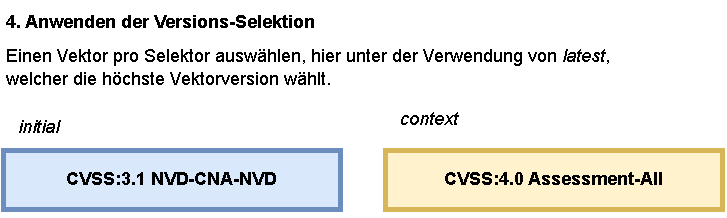
\includegraphics[width=0.7\textwidth, keepaspectratio]{res/grafiken/cvss-selection-process-selection-4}
    \caption{Anwenden der Versions-Selektion}
    \label{fig:cvss-selection-process-selection-4}
\end{figure}


\subsection{CVSS TypeScript Implementation} \label{subsec:projektbericht-loesungsweg-typescript-cvss-online-calculator}

Dieses Kapitel geht auf die Details hinter der CVSS-Implementierung\footnote{\url{https://github.com/org-metaeffekt/metaeffekt-universal-cvss-calculator}} in TypeScript ein, wie sie im Universal CVSS Calculator\footnote{\url{https://www.metaeffekt.com/security/cvss/calculator}} der {\metaeffekt} verwendet wird.
In Abbildung \ref{fig:cvss-ts-calculator-class-diagram} kann das Klassendiagramm der TypeScript-Klassen mit allen Exports und Imports gefunden werden, welche in diesem Kapitel erklärt werden.

\begin{figure}[htbp] % here, top, bottom, separate page
    \centering
    \makebox[\textwidth][c]{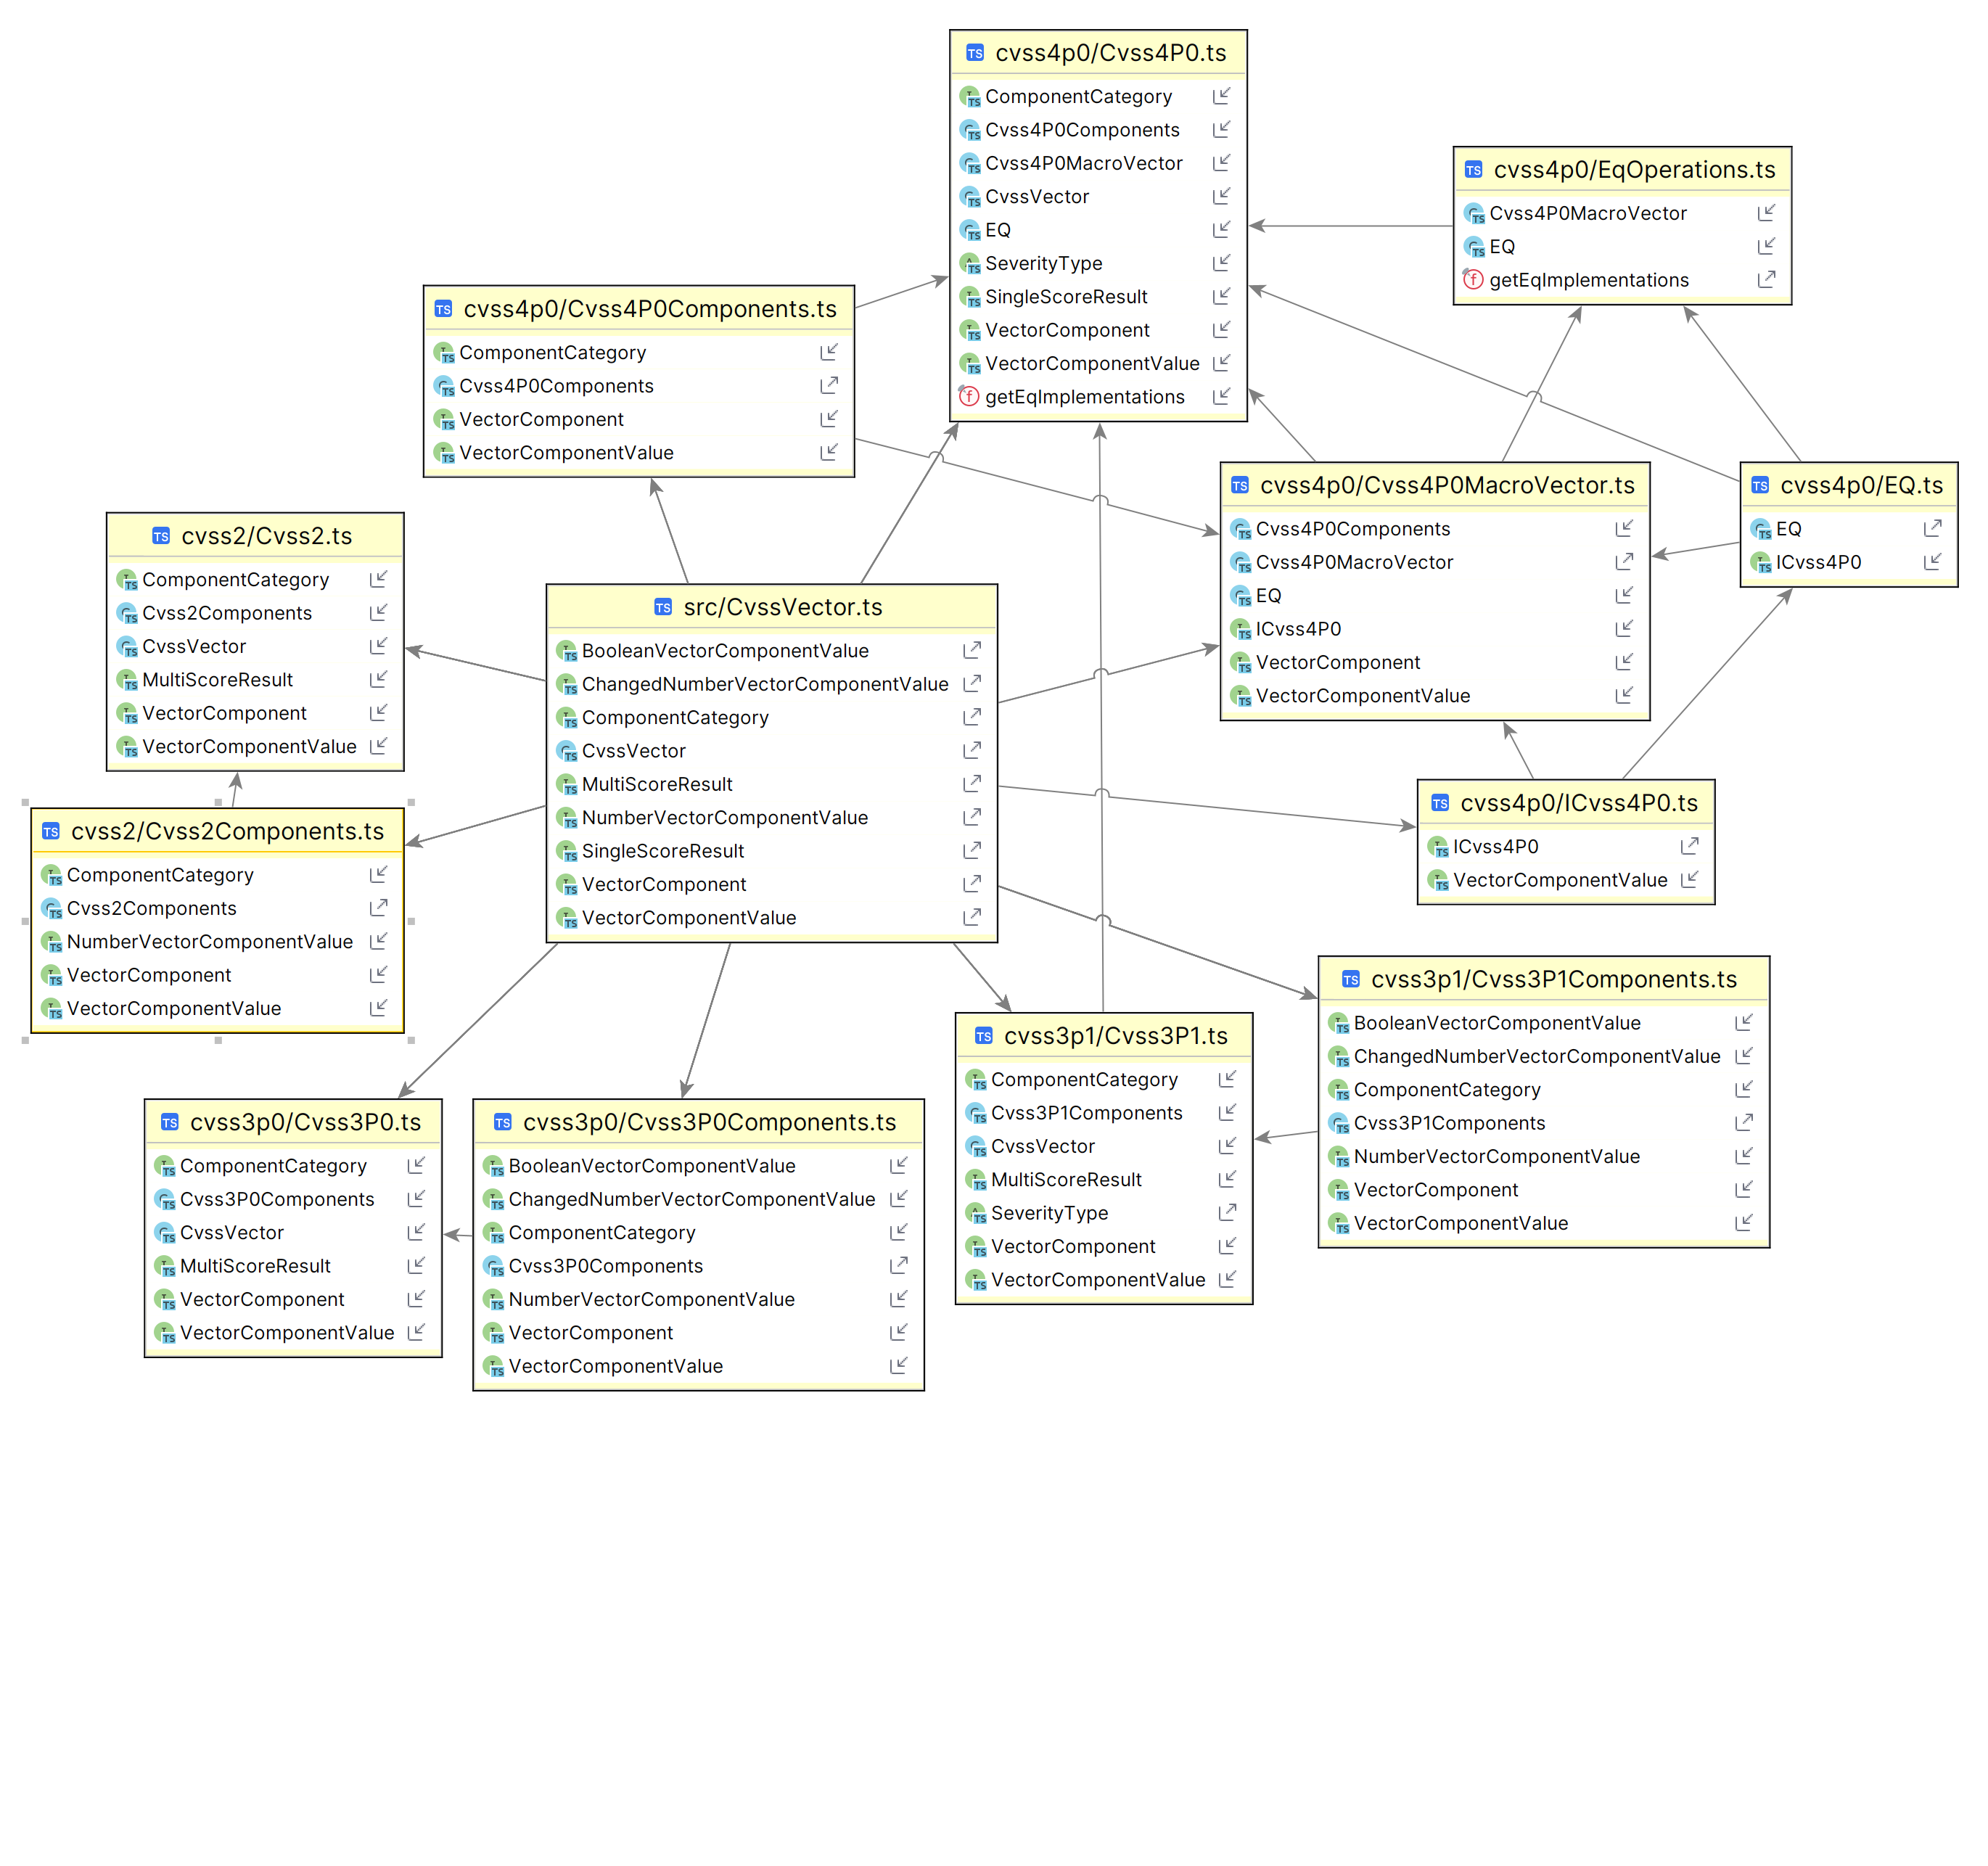
\includegraphics[width=1.2\textwidth, keepaspectratio]{res/grafiken/cvss-ts-calculator-class-diagram}}
    \caption{Klassendiagramm des CVSS-Rechners in TypeScript}
    \label{fig:cvss-ts-calculator-class-diagram}
\end{figure}

Da sich die Vektoren nur in ihren verwendeten Metriken, Metrikgruppen und der Score-Berechnung unterscheiden, kann recht viel der gemeinsamen Logik in eine Oberklasse \code{CvssVector} extrahiert werden.
In Listing \ref{lst:cvss-typescript-cvss-vector-class-attributes} wird ein Ausschnitt der recht schmalen Attributmenge und einigen relevanten Methoden gegeben.

\begin{lstlisting}[language=Java, label={lst:cvss-typescript-cvss-vector-class-attributes}, caption={CvssVector Klasse in TypeScript}, basicstyle=\scriptsize]
export abstract class CvssVector<R extends BaseScoreResult> {
    components: Map<VectorComponent<VectorComponentValue>, VectorComponentValue>;

    public abstract calculateScores(normalize: boolean): R;
    public abstract getVectorName(): string;
    public applyComponent(setComponent: VectorComponent<VectorComponentValue>, setValue: VectorComponentValue) { ... }
    public getComponent<T extends VectorComponentValue>(component: VectorComponent<T>): T { ... }
}
\end{lstlisting}

Generell ist das Schema jeder Berechnungsfunktion mit \code{calculateScores} gleich, denn es wird immer ein Objekt mit mindestens einem Overall-Score und je nach Vektorversion zusätzliche Scores konstruiert und zurückgegeben.
In Listing \ref{lst:cvss-typescript-cvss-3P1-calculateScores} wird dies anhand von CVSS 3.1 gezeigt, da diese Version einige Besonderheiten darstellt.
CVSS 3.1 hat unter anderem das Problem, dass der sog. \qt{Environmental} und \qt{Temporal} Score nicht auf eine Spanne von 0-10 normalisiert werden, sondern nur bis 6.0 oder 3.9 reichen.
Mit einem \code{normalize}-Parameter können diese scores auf die Spanne von 0-10 gemappt werden.
Zudem kann nicht immer jeder Score berechnet werden, denn zu den Scores müssen immer mindestens die entsprechenden Metriken vorhanden sein.

\begin{lstlisting}[language=Java, label={lst:cvss-typescript-cvss-3P1-calculateScores}, caption={CVSS 3.1 Score-Berechnung in TypeScript}, basicstyle=\scriptsize]
calculateScores(normalize: boolean = false): MultiScoreResult {
    const base = isBaseFullyDefined();
    const temp = isAnyTemporalDefined();
    const env = isAnyEnvironmentalDefined();
    return {
        base: base ? round(baseScore(), 1) : undefined,
        impact: base ? normalize(round(impactScore(), 1), normalize ? 6.0 : 10) : undefined,
        exploitability: base ? normalize(round(exploitabilityScore(), 1), normalize ? 3.9 : 10) : undefined,
        temporal: base && temp ? round(temporalScore(), 1) : undefined,
        environmental: base && env ? round(environmentalScore(), 1) : undefined,
        modifiedImpact: base && env ? normalize(round(Math.max(0, adjustedImpactScore()), 1), normalize ? 6.1 : 10) : undefined,
        overall: round(overallScore(), 1),
        vector: toString()
    };
}
\end{lstlisting}

Die einzelnen Score-Berechnungsmethoden wurden von der Spezifikation\footnote{\url{https://www.first.org/cvss/v3.1/specification-document\#CVSS-v3-1-Equations}} übernommen und ähneln sich alle stark.
Ein typisches Beispiel ist die Berechnung des Impact-Scores, bei der auf diverse Metriken (unterschiedlichen Datentyps) zugegriffen wird und diese mit weiteren konstanten Werten verrechnet werden.
In Listing \ref{lst:cvss-typescript-cvss-3P1-calculateExactImpactScore} ist der dazugehörige Code zu finden.
\begin{align*}
    \text{ISS} &= 1 - [ (1 - \text{Confidentiality}) \times (1 - \text{Integrity}) \times (1 - \text{Availability}) ] \\
    \text{If Scope is Unchanged:} & \quad 6.42 \times \text{ISS} \\
    \text{If Scope is Changed:} & \quad 7.52 \times (\text{ISS} - 0.029) - 3.25 \times (\text{ISS} - 0.02)^{15}
\end{align*}

\begin{lstlisting}[language=Java, label={lst:cvss-typescript-cvss-3P1-calculateExactImpactScore}, caption={CVSS 3.1 Impact Score-Berechnung in TypeScript}, basicstyle=\scriptsize]
public calculateExactImpactScore(): number {
    const iss = 1 - ((1 - getComponent(C).value) * (1 - getComponent(I).value) * (1 - getComponent(A).value));

    if (getComponent(S).value) return SCOPE_CHANGED_FACTOR * (iss - 0.029) - 3.25 * Math.pow(iss - 0.02, 15);
    else return SCOPE_UNCHANGED_FACTOR * iss;
}
\end{lstlisting}

\subsubsection{CVSS:4.0 TypeScript Implementierung} \label{subsec:projektbericht-loesungsweg-typescript-cvss-online-calculator-cvss-4P0}

Etwas anders verhält es sich mit der Version 4.0 von CVSS, welche nur einen einzigen Score berechnet und dazu keine statischen Formeln, sondern höhere mathematische Konzepte verwendet.
Laut der Dokumentation und Entwicklungsgeschichte von CVSS 4.0 \cite{CVSSv4.0Specification} wurden die 15 Millionen möglichen CVSS-Vektoren automatisiert in 270 Äquivalenzgruppen aufgeteilt und einer Expertengruppe mit 50 Teilnehmern bereitgestellt, die diese absolut dem Schweregrad entsprechend einordnen sollten.
Dadurch konnte eine durchschnittliche Liste an Vektoren mit aufsteigenden Schweregraden berechnet werden, welcher recht einfach linear die CVSS-Scores von 0 bis 10 statisch vergeben und in einer Lookup-Tabelle der Öffentlichkeit zur Verfügung gestellt wurde.
Bei der Berechnung der Scores wird nun der initiale Input-Vektor mit seinen 32 Metriken auf nur 6 Dimensionen über diverse Regeln auf einen sog. \qt{MakroVektor} reduziert, um durch eben diese Lookup-Tabelle einen entsprechenden Basis-Score zu erhalten.
Nun wären allerdings 270 Scores etwas wenig, um die Vielfalt und den Detailgrad aller 15 Millionen Kombinationen darzustellen.
Daher wird ein Interpolationschritt dahinter geschaltet, der den Großteil der Berechnungslogik einnimmt.

Die folgenden Formeln werden nicht im Standard aufgeführt, da dieser sich eher mit den Konzepten hinter der Berechnung beschäftigt und nicht mit den eigentlichen Berechnungsmethoden.
Die Formeln und Teile der Bezeichner wurden aus der Implementierung abgeleitet und die Konzepte entsprechend angepasst.

\begin{align*}
    \text{ScoreInterpolated}(V) &= \text{ScoreBase}(MV) - \text{Mean}(\text{ScoreEQ}) \\
    \text{ScoreEQ} &= \text{ProportionDistance}(V, EQ) \times \text{ScoreRange}(MV, EQ) \\
    \text{ProportionDistance}(V, EQ) &= \frac{\text{SeverityDistance}(V, \text{MacroVector})}{\text{Depth}(\text{MacroVector})}
\end{align*}

Um die Formeln zu verstehen, muss verstanden werden, dass es zwei unterschiedliche Skalen mit verschiedenen Bedeutungen gibt:

\begin{description}
    \item[Severity Distance Scale] Diese Skala ist mit den Vektormetriken und deren möglichen Werten verbunden.
    Eine Änderung von $\pm 1$ auf dieser Skala stellt eine Änderung eines einzelnen Metrikwerts um einen Wert nach oben oder unten dar (ernster, weniger ernst).
    \item[CVSS Score Scale] Sie quantifiziert die Schwere der Schwachstelle in einem Bereich von 0 bis 10, wobei höhere Werte auf schwerwiegendere Schwachstellen hinweisen.
    Die kleinste mögliche Änderung auf dieser Skala ist $0.1$.
\end{description}

Damit können die folgenden Werte und Formeln definiert werden:

\begin{itemize}[noitemsep]
    \item \textbf{MV} ist der aus dem ursprünglichen Vektor berechnete MakroVektor.
    \item \textbf{EQ} ist eine sog.\ Äquivalenzgruppe, die aus einer Menge an Definitionen für Kriterien, wann ein Vektor innerhalb dieser Gruppe ist und eine Liste der Vektoren mit den höchstmöglichen Scores die in dieser Gruppe sind, führt.
    \item \textbf{ScoreInterpolated$(V)$} ist der endgültig berechnete Score für den Vektor.
    \item \textbf{ScoreBase$(MV)$} ist der Score für den MacroVector, bestimmt durch Nachschlagen in der Tabelle.
    \item \textbf{Mean$(scores)$} berechnet den Durchschnittsscore über alle EQ (Äquivalenz)-Gruppen, die für den Vektor zutreffen.
    \item \textbf{ScoreEQ} ist eine Liste von proportionalen Score-Anpassungen für jede EQ-Gruppe, berechnet durch eine Unterformel.
    \item \textbf{ProportionDistance$(V, EQ)$} (severity distance scale) berechnet als die Severity Distance geteilt durch die Tiefe des MacroVectors für diese EQ-Gruppe, ergibt einen Wert zwischen 0 und 1.
    \item \textbf{SeverityDistance$(V, MacroVector)$} (severity distance scale) ist die Anzahl der Metrikwertänderungen, die benötigt werden, um den Vektor $V$ vom Vektor mit der höchsten Schwere innerhalb desselben MacroVectors zu erreichen.
    \item \textbf{Depth$(MacroVector)$} (severity distance scale) ist die Gesamtanzahl der Metrikwertänderungen innerhalb eines MacroVectors von seinem höchsten bis zu seinem niedrigsten Schwerevektor.
    Diese ist je nach MakroVektor unterschiedlich, da jeder unterschiedlich breit sein kann.
    \item \textbf{ScoreRange$(MV, EQ)$} (CVSS score scale) ist der Unterschied im Score zwischen dem höchsten und niedrigsten Schwerevektor innerhalb des MacroVectors für eine gegebene EQ-Gruppe.
    Sie repräsentiert die effektive Score-Spanne innerhalb eines MakroVektors.
\end{itemize}

In Listing \ref{lst:cvss-typescript-cvss-4P0-calculateOverallScore-pseudocode} wird der Pseudocode für die Berechnung des Scores gezeigt, wie er sonst in der Cvss4P0-Klasse gefunden werden kann.

\begin{lstlisting}[language=Java, label={lst:cvss-typescript-cvss-4P0-calculateOverallScore-pseudocode}, caption={CVSS 4.0 Score-Berechnung Pseudocode}, basicstyle=\scriptsize]
function calculateOverallScore(inputVector):
  if not isBaseFullyDefined(inputVector):
      return 0.0
  if isNoImpactOnSystem(inputVector):
      return 0.0

  eqOperations = getEqImplementations() // implementations for handling equivalence groups

  macroVector = getMacroVector(inputVector)
  performSafetyCheck(macroVector)
  macroVectorScore = lookupTableScore(macroVector)

  allHighestSeverityVectors = []
  for eqOp in eqOperations:
    allHighestSeverityVectors.add(eq.getHighestSeverityVectors(macroVector))

  highestSeverityVectorCombinations = generateCvssPermutations(allHighestSeverityVectors)
  if highestSeverityVectorCombinations is empty:
      return 0.0 // no max vectors found
  highestSeveritySeverityDistances = calculateSeverityDistances(highestSeverityVectorCombinations)

  meanScoreAdjustment = new AverageCalculator()
  for eqOp in eqOperations:
      nextLessSevereMacroVector = eqOp.deriveNextLowerMacro(macroVector)
      nextLowerMacroScore = eqOp.lookupScoresForNextLowerMacro(nextLessSevereMacroVector)
      availableSeverityReduction = macroVectorScore - nextLowerMacroScore

      macroVectorDepth = lookupMacroVectorDepth(eqOp, macroVector)
      severityDistanceFromThisToHighestSeverity = eqOp.sumSeverityDistances(highestSeveritySeverityDistances)

      if not isNaN(availableSeverityReduction) and macroVectorDepth != 0.0:
          percentageToNextSeverityDistance = severityDistanceFromThisToHighestSeverity / macroVectorDepth
          normalizedSeverityDistance = percentageToNextSeverityDistance * availableSeverityReduction
          meanScoreAdjustment.add(normalizedSeverityDistance)

  adjustedOriginalMacroVectorScore = macroVectorScore - meanScoreAdjustment.average()

  return adjustScoreWithinValidRange(adjustedOriginalMacroVectorScore)
\end{lstlisting}


